%%% The main file. It contains definitions of basic parameters and includes all other parts.

% Meta-data of your thesis (please edit)
\input metadata.tex

% Generate metadata in XMP format for use by the pdfx package
\input xmp.tex

%% Settings for single-side (simplex) printing
% Margins: left 40mm, right 25mm, top and bottom 25mm
% (but beware, LaTeX adds 1in implicitly)
\documentclass[12pt,a4paper]{report}
\setlength\textwidth{145mm}
\setlength\textheight{247mm}
\setlength\oddsidemargin{15mm}
\setlength\evensidemargin{15mm}
\setlength\topmargin{0mm}
\setlength\headsep{0mm}
\setlength\headheight{0mm}
% \openright makes the following text appear on a right-hand page
\let\openright=\clearpage

%% Settings for two-sided (duplex) printing
% \documentclass[12pt,a4paper,twoside,openright]{report}
% \setlength\textwidth{145mm}
% \setlength\textheight{247mm}
% \setlength\oddsidemargin{14.2mm}
% \setlength\evensidemargin{0mm}
% \setlength\topmargin{0mm}
% \setlength\headsep{0mm}
% \setlength\headheight{0mm}
% \let\openright=\cleardoublepage

%% If the thesis has no printed version, symmetric margins look better
% \documentclass[12pt,a4paper]{report}
% \setlength\textwidth{145mm}
% \setlength\textheight{247mm}
% \setlength\oddsidemargin{10mm}
% \setlength\evensidemargin{10mm}
% \setlength\topmargin{0mm}
% \setlength\headsep{0mm}
% \setlength\headheight{0mm}
% \let\openright=\clearpage

%% Generate PDF/A-2u
\usepackage[a-2u]{pdfx}

%% Prefer Latin Modern fonts
\usepackage{lmodern}
% If we are not using LuaTeX, we need to set up character encoding:
\usepackage{iftex}
\ifpdftex
\usepackage[utf8]{inputenc}
\usepackage[T1]{fontenc}
\usepackage{textcomp}
\fi

%% Further useful packages (included in most LaTeX distributions)
\usepackage{amsmath}        % extensions for typesetting of math
\usepackage{amsfonts}       % math fonts
\usepackage{amsthm}         % theorems, definitions, etc.
\usepackage{array}          % multicolumns
\usepackage{bm}             % boldface symbols (\bm)
\usepackage{booktabs}       % improved horizontal lines in tables
\usepackage{caption}        % custom captions of floating objects
\usepackage{dcolumn}        % improved alignment of table columns
\usepackage{floatrow}       % custom float environments
\usepackage{graphicx}       % embedding of pictures
\usepackage{indentfirst}    % indent the first paragraph of a chapter
\usepackage[nopatch=item]{microtype}   % micro-typographic refinement
\usepackage{paralist}       % improved enumerate and itemize
\usepackage{subcaption}     % support for multiple images within one figure
\usepackage[nottoc]{tocbibind} % makes sure that bibliography and the lists
			    % of figures/tables are included in the table
			    % of contents
\usepackage{xcolor}         % typesetting in color

% The hyperref package for clickable links in PDF and also for storing
% metadata to PDF (including the table of contents).
% Most settings are pre-set by the pdfx package.
\hypersetup{unicode}
\hypersetup{breaklinks=true}

% Packages for computer science theses
\usepackage{algpseudocode}  % part of algorithmicx package
\usepackage{algorithm}
\usepackage{fancyvrb}       % improved verbatim environment
\usepackage{listings}       % pretty-printer of source code

% You might want to use cleveref for references
% \usepackage{cleveref}

% Set up formatting of bibliography (references to literature)
% Details can be adjusted in macros.tex.
%
% BEWARE: Different fields of research and different university departments
% have their own customs regarding bibliography. Consult the bibliography
% format with your supervisor.
%
% The basic format according to the ISO 690 standard with numbered references
\usepackage[natbib,style=iso-numeric,sorting=none]{biblatex}
% ISO 690 with alphanumeric references (abbreviations of authors' names)
%\usepackage[natbib,style=iso-alphabetic]{biblatex}
% ISO 690 with references Author (year)
%\usepackage[natbib,style=iso-authoryear]{biblatex}
%
% Some fields of research prefer a simple format with numbered references
% (sorting=none tells that bibliography should be listed in citation order)
%\usepackage[natbib,style=numeric,sorting=none]{biblatex}
% Numbered references, but [1,2,3,4,5] is compressed to [1-5]
%\usepackage[natbib,style=numeric-comp,sorting=none]{biblatex}
% A simple format with alphanumeric references:
%\usepackage[natbib,style=alphabetic]{biblatex}

% Load the file with bibliography entries
\addbibresource{bibliography.bib}

% Our definitions of macros (see description inside)
\input macros.tex

%%% Title page and various mandatory informational pages
\begin{document}
%%% Title page of the thesis and other mandatory pages

%%% Inscriptions at the opening page of the hard cover

% We usually do not typeset the hard cover, but if you want to do it, change \iffalse to \iftrue
\iffalse

\pagestyle{empty}
\hypersetup{pageanchor=false}
\begin{center}

\large
Charles University

\medskip

Faculty of Mathematics and Physics

\vfill

{\huge\bf\ThesisTypeTitle}

\vfill

{\huge\bf\ThesisTitle\par}

\vfill
\vfill

\hbox to \hsize{\YearSubmitted\hfil \ThesisAuthor}

\end{center}

\newpage\openright
\setcounter{page}{1}

\fi

%%% Title page of the thesis

\pagestyle{empty}
\hypersetup{pageanchor=false}
\begin{center}

\centerline{\mbox{
\includegraphics[width=166mm]{../img/logo-en.pdf}}}

\vspace{-8mm}
\vfill

{\bf\Large\ThesisTypeTitle}

\vfill

{\LARGE\ThesisAuthor}

\vspace{15mm}

{\LARGE\bfseries\ThesisTitle\par}

\vfill

\Department

\vfill

{
\centerline{\vbox{\halign{\hbox to 0.45\hsize{\hfil #}&\hskip 0.5em\parbox[t]{0.45\hsize}{\raggedright #}\cr
Supervisor of the \ThesisTypeName{} thesis:&\Supervisor \cr
\ifx\ThesisType\TypeRig\else
\noalign{\vspace{2mm}}
Study programme:&\StudyProgramme \cr
\fi
}}}}

\vfill

Prague \YearSubmitted

\end{center}

\newpage

%%% A page with a solemn declaration to the thesis

\openright
\hypersetup{pageanchor=true}
\vglue 0pt plus 1fill

\noindent
I declare that I carried out this \ThesisTypeName{} thesis on my own, and only with the cited
sources, literature and other professional sources.
I understand that my work relates to the rights and obligations under the Act No.~121/2000 Sb.,
the Copyright Act, as amended, in particular the fact that the Charles
University has the right to conclude a license agreement on the use of this
work as a school work pursuant to Section 60 subsection 1 of the Copyright~Act.

\vspace{10mm}

\hbox{\hbox to 0.5\hsize{%
In \hbox to 6em{\dotfill} date \hbox to 6em{\dotfill}
\hss}\hbox to 0.5\hsize{\dotfill\quad}}
\smallskip
\hbox{\hbox to 0.5\hsize{}\hbox to 0.5\hsize{\hfil Author's signature\hfil}}

\vspace{20mm}
\newpage

%%% Dedication

\openright

\noindent
\Dedication

\newpage

%%% Mandatory information page of the thesis

\openright
{\InfoPageFont

\vtop to 0.5\vsize{
\setlength\parindent{0mm}
\setlength\parskip{5mm}

Title:
\ThesisTitle

Author:
\ThesisAuthor

\DeptType:
\Department

Supervisor:
\Supervisor, \SupervisorsDepartment

Abstract:
\Abstract

Keywords:
{\def\sep{\unskip, }\ThesisKeywords}

\vfil
}

% In Czech study programmes, it is mandatory to include Czech meta-data:

\ifx\StudyLanguage\LangCS

\vtop to 0.49\vsize{
\setlength\parindent{0mm}
\setlength\parskip{5mm}

Název práce:
\ThesisTitleCS

Autor:
\ThesisAuthor

\DeptTypeCS:
\DepartmentCS

Vedoucí bakalářské práce:
\Supervisor, \SupervisorsDepartmentCS

Abstrakt:
\AbstractCS

Klíčová slova:
{\def\sep{\unskip, }\ThesisKeywordsCS}

\vfil
}

\fi

}

\newpage

%%% Further pages will be numbered
\pagestyle{plain}

%%% A page with automatically generated table of contents of the thesis

\tableofcontents

%%% Each chapter is kept in a separate file
\chapter*{Introduction}
\addcontentsline{toc}{chapter}{Introduction}


\chapter{Problem description}\label{ch:problem}
\section{Input description}

The following instance data define a problem instance.

\begin{itemize}
    \item Set of customer requests $R$, where every request consists of its unique identifier $id$, the earliest time of departure $t_d$ (number of seconds from the start of the simulation), group size (number of passengers in the group), coordinates of the group's departure location, and coordinates of the group's arrival location. The size of any group cannot exceed the capacity of the largest available bus.
    \item The coordinates of the \textit{depot}
    \item The \textit{bus type} available from the depot. The bus type must include the capacity of the bus $c$, the operational cost of the bus per kilometer $o$, and the one-time fee for using the bus $f$.
    \item Distances between each point (in meters).
    \item Travel times between each point (in seconds).
\end{itemize}

\section{Solution} \label{sec:solution}

The solution is a set of routes. Each route is given as a list of group indices in the order the bus handles their pick-ups and drop-offs.

For a solution to be valid, the following constraints must hold.

\begin{enumerate}[(1)]\label{constraints}
    \setlength\itemsep{0pt}
    \item Each group is handled by exactly one bus.
    \item Each group must be picked up and dropped off by a bus exactly once and as a whole.
    \item No bus carries more passengers than its capacity allows it to.
\end{enumerate}

This means that each group can appear in only one route. Each group's index must be included in its corresponding route \textit{exactly twice} - the first occurrence marks the pick-up, and the second occurrence marks the drop-off.

Every route needs to start and end at the depot. Since only one is available, it is implicitly added to every route's beginning and end.

\section{Objective function}
\label{sec:objective}

Since the goal is to minimize the costs, they form the foundation of the function. With $S$ being the solution, $r$ a route within the solution, $r_i$ the $i$th stop on the route, and $d(r_i, r_j)$ the distance between stops $r_i$ and $r_j$ in kilometers, the total operational cost of the buses is given by the equation
\begin{equation}\label{eq:objective_costs}
    \text{operational cost} \equiv \sum_{r \in S} ( f + o \cdot \sum_{i=1}^{|r|}d(r_{i-1},r_{i}))
\end{equation}


We must also account for the group's \textit{delays} when evaluating a solution. The delay for each group is calculated as the difference between the time we drop the group off and the \textit{expected arrival time}, which is defined as the sum of the group's departure time and the travel time between the group’s departure and destination points.

We represent the ``satisfaction'' of the customers by the equation
\begin{equation}\label{eq:objective_satisfaction}
     \text{satisfaction cost} \equiv \sum_{g \in groups} p_t \cdot d_g^2
\end{equation}
where $p_t$ is the penalty constant for late arrival and $d_g$ is the group's delay. The group's delay is squared to penalize larger delays more. The penalty constant is a hyperparameter and depends on the priority of handling all the customers as soon as possible at the expense of higher operational costs.

The objective function is then the sum of the \textit{operational} and \textit{satisfaction} cost.

\begin{equation}\label{eq:objective}
    \sum_{r \in S} ( f + o \cdot \sum_{i=1}^{|r|}d(r_{i-1},r_{i})) + \sum_{g \in groups} p_t \cdot d_g^2
\end{equation}

\section{Input data generation}

We create our own benchmark data to compare the algorithms presented in the thesis. We have two basic dataset types, \textit{uniformly distributed} and \textit{commute}.

Given an OpenStreetMaps area, the number of requests to generate, the maximum size of a group in a request, and the latest possible departure time of a group, the \textit{uniformly distributed} generator creates requests where departure and destination coordinates are a randomly chosen public transport platform in the given area. The departure times and group sizes are chosen randomly. The number of platforms to sample from can be limited to force multiple customers to use the same platform for departure/destination. The depot is also randomly chosen from the available platforms, and the available bus type's \textit{capacity}, \textit{operational cost per km}, and \textit{fixed cost for usage} is given as a parameter.

The \textit{commute} generator generates requests similarly to the \textit{uniformly distributed generator} but takes three OpenStreetMaps areas instead, an \textit{area from}, \textit{area to}, and a \textit{depot area}. The departure coordinates are randomly chosen platforms from \textit{area from}, and destination coordinates are randomly chosen platforms from \textit{area to}. The depot coordinates are randomly chosen from the platforms in the \textit{depot area}. We can also use a \textit{two-way} parameter, which makes the generator also generate requests from \textit{area to} to \textit{area from}. The departure times for both directions are still randomly generated based on the latest possible departure time.

The customer requests are stored in \textit{GeoJSON} file, whose structure is described in detail in the attached \textit{JSON schema}.

We must also generate the \textit{distance} and \textit{duration} matrices. We use the Open Source Routing Machine (\textit{OSRM}) API \cite{luxen-vetter-2011}, which has a \textit{table service} that can generate both matrices based on a list of coordinates. The matrices are stored in separate \textit{CSV} files.

\iffalse

\section{Stuff to sort}

\begin{itemize}
    \item Since \textit{DARP} is a real-world problem, we will make some simplifications to the problem to simplify the problem's simulation. We won't constrain or penalize route lengths (we can assume that the buses can refill fuel between stops with no time penalty). We will also mostly ignore most of the needs of the bus driver, such as compulsory time breaks after driving for a certain amount of time or having limited working hours. \xxx{Probably move to the introduction}
\end{itemize}

\fi
\chapter{Optimization}

\section{Genetic algorithm}

The concept of genetic algorithms to solve computationally hard problems was first presented by John Holland \cite{Holland:1975}. Starting with a \textit{population} formed with initial (in most cases random) solutions (called \textit{individuals}), \textit{crossover} and \textit{mutation} operators are applied to gradually improve the fitness score of the population and thus find the best individual overall.

The most essential thing when designing a specific genetic algorithm is the encoding of an individual. Based on the encoding, we need to choose the genetic operators - \textit{crossover} and \textit{mutation}. The \textit{crossover} operator takes two random individuals (\textit{parents}) from the population and uses them to create two new individuals, which combine the properties of the parents. The \textit{mutation} operator takes only one individual and makes a change within him. The change should usually be small and can be either completely random or try to improve the individual using some heuristic (called a \textit{smart mutation}). The operators are performed on an individual or pair of individuals with a given probability (so in each generation, only some individuals participate in crossover or are mutated).

After the operators are applied, the new population is created using the \textit{selection}. In our cases, the selection can either be a \textit{roulette wheel selection} or a \textit{tournament selection}. In the \textit{roulette wheel selection}, we randomly sample individuals from the current population, but the individuals are weighted using their fitness value. When using the \textit{tournament selection}, we take $t$ (usually 2 or 3) random individuals from the population and compare their fitness values. The best one is chosen and added to the new population. This process is repeated until the new population is fully populated.

Apart from using the \textit{roulette wheel} or \textit{tournament} selection, we employ a strategy called \textit{elitism}. After the new population is sampled, we choose $n$ individuals randomly and replace them with the first $n$ best individuals from the old population. This ensures that the best individual in each population survives into the next generation.

\subsection{Individual as routes of stops}

\subsubsection{Coding of an individual}

The individual is encoded as a list of routes, where each route is a \textbf{list of stops} in the order the bus visits them.

Transforming the individual into a solution is done by simulation.  We simulate every route - at each stop, we pick up any group waiting for the bus at that stop and drop off every group present on the bus that can be dropped off. If multiple groups are waiting at the stop, but not all can fit into the bus, we prioritize the groups that are waiting longer. At the route end, if any groups are left on the bus, we drop them off in the order of their departure time and return to the depot. After all route simulations are completed, we create another route by taking all the groups not picked up by any bus, picking them up, and immediately dropping them off in the order of departure time. This ensures that the simulation returns a valid solution.

The difference between the encoding of a solution and our individual is that the individual uses stops instead of groups to encode a route. The main reason for introducing this change was that maintaining the correctness of the solution after performing the genetic operators on it would be problematic. Making a (semi-)random change in the individual could easily end up in the violation of constraints \hyperref[constraints]{(2)} or \hyperref[constraints]{(3)}. Using stops instead of groups eliminates the problem of invalidating an individual since there is no invalid individual.

\subsubsection{Fitness function}

The fitness function is evaluated by transforming the individual to a solution and calculating the objective function equation \ref{eq:objective}.

\subsubsection{Initial population}

We present two ways to create the initial population - \textit{random} and \textit{greedy}.

The \textit{random} individual generator generates random sequences of stops and takes as a parameter the number of buses to use and the maximum allowed length of a route.

The \textit{greedy} generator tries to generate already feasible routes. At each stop, we generate a set of reasonable next actions - picking up a new group or dropping off a group present on the bus. When considering groups to pick up, we only consider those whose departure time is close to the arrival time to their pick-up stop. For this, the generator takes a parameter defining how large this \textit{time window} should be. If no more options exist, the bus ends the route by traveling to the depot. The generator can also be limited by parameters that define the maximum number of buses that can be used or the maximum number of groups that can be picked up within one route.

\subsubsection{Crossover}

We use a simple \textit{one-point crossover}. We take \textbf{one} random route from each individual, select a \textit{crossover point}, and swap the right parts of the routes between the individuals.

We decided to use the crossover on only one of the routes for each individual. This is because even a change in one route is usually quite a big change - it can easily result in not picking up or dropping off some groups and, therefore, making the new individual largely penalized. However, it also makes the genetic algorithm much more exploratory.

\subsubsection{Mutation}

Unlike crossover, we have many options on what mutation operators to choose. We decided to implement many of them as \textit{``submutations''} and randomly choose one of them at each mutation. The probability of each \textit{``submutation''} is determined by its weight, and the weights are set before an experiment as hyper-parameters.

The possible \textit{``submutations''} are:
\begin{itemize}
    \setlength\itemsep{0pt}
    \item Delete a random stop from a randomly chosen route.
    \item Add a random stop to a randomly chosen route.
    \item Change a stop to a random one in a randomly chosen route.
    \item Reverse a random sub-route of a randomly chosen route. This is the main source of changing the stops' order.
    \item Shuffle the routes within the solution. This can greatly impact the simulation when evaluating the fitness function since each group is picked up by the first bus (in the simulation order) that arrives at their stop at the right time. If more buses travel through the same stop, groups on that stop can be picked up by a completely different bus.
    \item ``Smart mutation'' - depending on the quality of the individual, it either tries to add an ``unhandled'' group to a random route, or it tries to perform a swap of a group between 2 routes. In both cases, we need to insert to a route both pick-up and drop-off points. The maximum distance between these points is given as a parameter.
\end{itemize}

\subsubsection{Hyper-parameters}

The hyper-parameter values largely influence the behavior of the algorithm. We perform a series of experimental measures to find the optimal values for the most important ones and those that are hard to guess beforehand.

\begin{figure}[b]
    \centering
    \begin{subfigure}[b]{0.45\textwidth}
        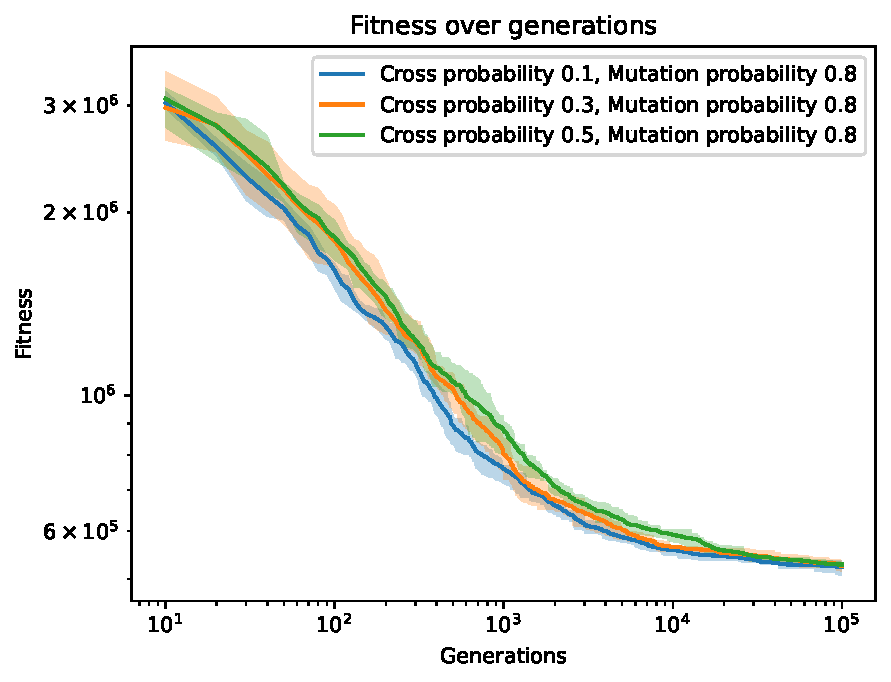
\includegraphics[width=\textwidth]{img/evo1_cross_prob_random.pdf}
        \caption{Randomly distributed data}
        \label{fig:evo1_cross_random}
    \end{subfigure}
    \begin{subfigure}[b]{0.45\textwidth}
        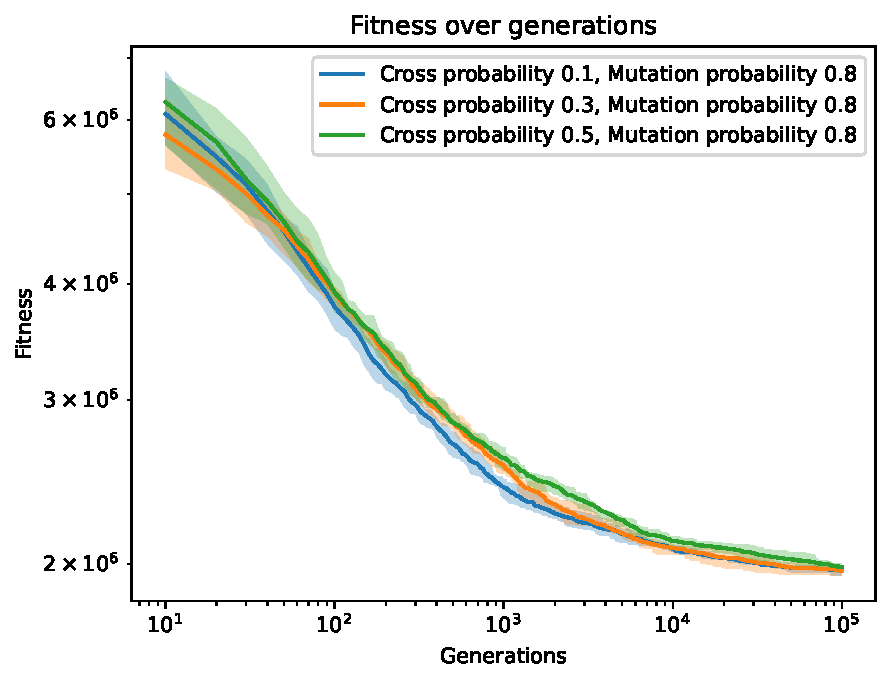
\includegraphics[width=\textwidth]{img/evo1_cross_prob_commute.pdf}
        \caption{Long distance commute data}
        \label{fig:evo1_cross_commute}
    \end{subfigure}
    \caption{Individual as stops - crossover probability}
    \label{fig:evo1_cross}
\end{figure}

\label{experiment_graph_description}
We start with the crossover probability. We conduct three experiments with probability values $0.1$, $0.3$, and $0.5$. Each experiment runs the genetic algorithm 10 times. In figure \ref{fig:evo1_cross}, for each experiment, the mean fitness of the 10 runs is depicted as the primary line, accompanied by the first and third quartiles represented as a translucent region. Both $x$ and $y$ axes are logarithmic. The figure shows that while the difference is marginal, the lowest probability, $0.1$, converged the fastest and gave the best result overall on both datasets.

The one-point crossover is not suitable for the commute data. Since the bus needs to pick up groups at one area first and then travel to the second area, cutting the route in half is not logical. However, since on the randomly distributed data, the probability $0.3$ gave very similar results to the $0.1$ probability and since the crossover focuses on \textit{exploration} rather than \textit{exploitation}, keeping the slightly higher probability on longer runs on randomly distributed datasets might work better.

The rest of the hyper-parameter values were chosen similarly and are shown in the table \ref{tab:evo_stops_hyperparams}.

\begin{table}[h]
    \centering
    \begin{tabular}{lcc}
         & Random & Commute \\
        \hline
        Mutation probability & \multicolumn{2}{c}{0.8} \\
        Crossover probability & 0.3 & 0.1 \\
        Selection & \multicolumn{2}{c}{tournament ($t=2$)} \\
        Create individual function & \multicolumn{2}{c}{greedy} \\
        Smart mutation weight & \multicolumn{2}{c}{12} \\
        Reverse a route weight & \multicolumn{2}{c}{3} \\
        Add/Delete/Change a stop randomly weight & \multicolumn{2}{c}{9} \\
        Shuffle individual weight & \multicolumn{2}{c}{2} \\
        Smart mutation maximum pick-up-drop-off distance & 4 & 50 \\
    \end{tabular}
    \caption{Individual as stops - hyper-parameter settings}
    \label{tab:evo_stops_hyperparams}
\end{table}

\subsection{Individual as separate clustering and routing}

\subsubsection{Coding of an individual}

The individual consists of two parts: the mapping between a group and a route, which \textit{clusters} the groups, and the order in which the groups are picked up and dropped off.

The mapping is defined by an array, where the array indices represent the \textit{group identifiers} and the values represent the \textit{identifier of the route that handles the group}. The maximum number of routes is given as a parameter to limit the number of routes used.

The order of pick-ups and drop-offs is defined by an array, where every group occurs twice; the first occurrence marks the pick-up, and the second marks the drop-off.

To transform an individual into a solution, for each route, we first determine which groups are handled by that route, and then we construct the route by picking the group's indices in the order they are present in the individual's order-defining array.

\subsubsection{Fitness function}

The fitness function is evaluated by transforming the individual to a solution and calculating the objective function equation \ref{eq:objective}.

\subsubsection{Initial population}

We generate the initial solutions randomly - given the maximum number of routes, we assign each group to a random route, and the order of the groups is created by a random shuffle.

\subsubsection{Crossover}

In the crossover, we only cross the order of handling the groups. We first transform the order array into a permutation by adding $|R|$ to every second occurrence of each group. On this permutation, we can use classic combinatorial crossovers, e. g. the \textit{Partially Mapped Crossover (PMX)} \cite{Goldberg1985AllelesLA}, the \textit{Order Crossover (OX)} \cite{Davis1985ApplyingAA}, or the \textit{Cyclic Crossover (CX)} \cite{Oliver1987ASO}. We then transform the permutation back to the order array by subtracting $|R|$ from every second occurrence of each group.

The concrete choice of which combinatorial crossover is used on the permutation is a hyper-parameter. The implementations of these crossovers are used from the \textit{Evolutionary.jl} library \cite{art_2022_5851574}.

\subsubsection{Mutation}

Mutation has multiple options for changing the individual. It can change the route assignment by either swapping two random groups between routes or assigning a random route to a random group, or it can change the order by either reversing a part of the order array or swapping two values in the order array.

\subsubsection{Hyper-parameters}

The hyper-parameter settings for both \textit{random} and \textit{commute} dataset types were chosen experimentally and are shown in the table \ref{tab:evo_cr_hyperparams}.

\begin{table}[h]
    \centering
    \begin{tabular}{lcc}
         & Random & Commute \\
        \hline
        Mutation probability & \multicolumn{2}{c}{0.8} \\
        Crossover probability & 0.4 & 0.6 \\
        Crossover type & \multicolumn{2}{c}{PMX} \\
        Selection & \multicolumn{2}{c}{tournament ($t=2$)} \\
        Mutate route assignments probability & \multicolumn{2}{c}{0.5} \\
        Swap two groups between routes mutation probability & \multicolumn{2}{c}{0.5} \\
        Reverse a part of the order array mutation probability & \multicolumn{2}{c}{0.7} \\ 
    \end{tabular}
    \caption{Individual as cluster and route - hyper-parameter settings}
    \label{tab:evo_cr_hyperparams}
\end{table}

\subsection{Individual as only clustering with heuristic routing}

\subsubsection{Coding of an individual}

The individual comprises only the mapping between the groups and the routes, which is stored in an array, where the array indices represent the group identifiers and the values represent the identifier of the route that handles the group.

To convert an individual into a solution, we first divide the groups into routes based on the individual. The order in which we handle the groups within a route is then calculated based on a greedy space-time nearest neighbor heuristic described by Baugh et al. \cite{doi:10.1080/03052159808941240}.

The heuristic is based on assigning a \textit{cost} to each movement, which is calculated as a weighted sum of the travel time between the stops and the \textit{time window violation} - how much ``on time'' did we pick up/drop off passengers. We define the beginning of a group's \textit{time window} as the sum of the group's departure time and the travel time between departure and destination points. The time window end is then the sum of the travel time multiplied by a \textit{time window size} parameter and the group's departure time. The \textit{violation} is then calculated as how ``far'' we are from the time window in seconds.

When evaluating the route, we first find $d$ ``cheapest'' possible options to travel to, where $d$ is a heuristic depth parameter. We only choose those options that would not violate any constraints defined in the section \ref{sec:solution}. For each of the options, we then try to determine the cost of the resulting route if we choose this option. We do this by evaluating the cost of a route where, for $d$ stops, we would always choose the ``cheapest'' available option. Based on the costs of these routes, we then choose the best option overall. We then repeat this process until no options are available and all groups are picked up and dropped off.

\subsubsection{Fitness function}

The fitness function is evaluated by transforming the individual to a solution and calculating the objective function equation \ref{eq:objective}.

\subsubsection{Initial population}

We generate the initial solutions randomly - given the maximum number of routes to use, we assign each group to a random route.

\subsubsection{Crossover}

We use a uniform crossover - for each of the two individuals, we go through the group-routes assignment, and with a given probability, we change the current assignment to the one in the second individual.

\subsubsection{Mutation}

The mutation swaps two random groups between their routes or assigns a random route to a random group.

\subsubsection{Hyper-parameters}

The hyper-parameter settings for both \textit{random} and \textit{commute} dataset types were chosen experimentally and are shown in the table \ref{tab:evo_ch_hyperparams}.

\begin{table}[ht]
    \centering
    \begin{tabular}{lcc}
         & Random & Commute \\
        \hline
        Mutation probability & \multicolumn{2}{c}{x} \\
        Crossover probability & \multicolumn{2}{c}{x} \\
        Selection & \multicolumn{2}{c}{x} \\
        Travel time weight in heuristic cost & \multicolumn{2}{c}{x} \\
        Time window violation weight in heuristic cost & \multicolumn{2}{c}{x} \\
        Time window size & \multicolumn{2}{c}{x} \\
        Uniform crossover switch assignment probability & \multicolumn{2}{c}{x} \\
        Swap two groups between routes mutation probability & \multicolumn{2}{c}{x} \\
    \end{tabular}
    \caption{Individual as only clustering with heuristic routing - hyper-parameter settings}
    \label{tab:evo_ch_hyperparams}
\end{table}

\section{Ant Colony Optimization}

\xxx{General meta-heuristics description}

\subsection{Individual as the solution itself}

\xxx{todo}

\iffalse

\subsubsection*{Coding of an individual:}
The individual is represented as a list of routes, where each route is an ordered list of groups. Each group is represented twice, once for the pick-up and once for the drop-off. Each route implicitly starts and ends at the depot.

\subsubsection*{Pheromone matrix}
The pheromone matrix is of size $2|G| \times 2|G| + 1$, where $G$ is the set of all groups. For each group with id $i$, the pheromone at index $2i - 1$ represents the probability of the group being picked up, and the pheromone at index $2i$ represents the likelihood of the group being dropped off. The last element of the matrix represents the probability of the bus moving to the depot (and thus ending its route).

\subsubsection*{Fitness function:}
The fitness function is calculated similarly to the genetic algorithm approach, with the only difference being that the routes of the individual are now encoded as lists of groups (where each group is represented twice, once for the pick-up and once for the drop-off), rather than lists of stops.

\subsubsection*{Attractiveness:}
An essential part of the ACO algorithm is the "attractiveness" - a simple heuristic value for each edge in the graph. Here, the attractiveness is calculated as the sum of the inverse of the distance and the inverse of the difference between the group's departure time and the time the bus arrives at the stop. Additionally, attractiveness is raised by a constant parameter value if the edge represents dropping off a group waiting in the bus (this tries to minimize the delays by dropping off groups as soon as possible). Also, when the attractiveness is calculated for the depot, it is raised by a parameter value (usually the length of the route multiplied by some parametric constant) to encourage the bus to return to the depot (and avoid making the routes too long).

\subsubsection*{Constructing new solutions:}
For every ant, we generate a solution as a list of routes. Each route starts at the depot. At each stop, the set of available subsequent nodes is calculated as a union of pick-up nodes for groups not picked up by any bus yet and drop-off nodes for groups in the bus. If there are no groups on the bus, the depot node is added to the set of available nodes instead (this ensures that the bus cannot end its route with passengers still onboard). Each probability is then calculated (as $pheromone^\alpha \cdot attractivness^\beta$), and the next stop is chosen using the roulette wheel selection. New routes are then constructed by repeating this process until all groups are handled

\fi
\chapter{Experimental results}

\chapter*{Conclusion}
\addcontentsline{toc}{chapter}{Conclusion}


%%% Bibliography
%%% Bibliography (literature used as a source)
%%%
%%% We employ bibTeX to construct the bibliography. It processes
%%% citations in the text (e.g., the \cite{...} macro) and looks up
%%% relevant entries in the bibliography.bib file.
%%%
%%% The \bibliographystyle command selects, which style will be used
%%% for references from the text. The argument in curly brackets is
%%% the name of the corresponding style file (*.bst). Both styles
%%% mentioned in this template are included in LaTeX distributions.

\bibliographystyle{plainnat}    %% Author (year)
% \bibliographystyle{unsrt}     %% [number]

\renewcommand{\bibname}{Bibliography}

%%% Generate the bibliography. Beware that if you cited no works,
%%% the empty list will be omitted completely.

\bibliography{bibliography}

%%% If case you prefer to write the bibliography manually (without bibTeX),
%%% you can use the following. Please follow the ISO 690 standard and
%%% citation conventions of your field of research.

% \begin{thebibliography}{99}
%
% \bibitem{lamport94}
%   {\sc Lamport,} Leslie.
%   \emph{\LaTeX: A Document Preparation System}.
%   2nd edition.
%   Massachusetts: Addison Wesley, 1994.
%   ISBN 0-201-52983-1.
%
% \end{thebibliography}


%%% Figures used in the thesis (consider if this is needed)
% \listoffigures

%%% Tables used in the thesis (consider if this is needed)
%%% In mathematical theses, it could be better to move the list of tables to the beginning of the thesis.
% \listoftables

%%% Abbreviations used in the thesis, if any, including their explanation
%%% In mathematical theses, it could be better to move the list of abbreviations to the beginning of the thesis.
\chapwithtoc{List of Abbreviations}
\begin{itemize}
    \item \textbf{DARP} - Dial-A-Ride Problem
\end{itemize}

%%% Doctoral theses must contain a list of author's publications
\ifx\ThesisType\TypePhD
\chapwithtoc{List of Publications}
\fi

%%% Attachments to the thesis, if any. Each attachment must be referred to
%%% at least once from the text of the thesis. Attachments are numbered.
%%%
%%% The printed version should preferably contain attachments, which can be
%%% read (additional tables and charts, supplementary text, examples of
%%% program output, etc.). The electronic version is more suited for attachments
%%% which will likely be used in an electronic form rather than read (program
%%% source code, data files, interactive charts, etc.). Electronic attachments
%%% should be uploaded to SIS. Allowed file formats are specified in provision
%%% of the rector no. 72/2017. Exceptions can be approved by faculty's coordinator.
\appendix
\chapter{Attachments}

%\usepackage{listings}
%\usepackage{xcolor}

\colorlet{punct}{red!60!black}
\definecolor{background}{HTML}{FCFCFC}
\definecolor{delim}{RGB}{20,105,176}
\colorlet{numb}{magenta!60!black}

\lstdefinelanguage{json}{
    basicstyle=\normalfont\ttfamily,
    numbers=left,
    numberstyle=\scriptsize,
    stepnumber=1,
    numbersep=8pt,
    showstringspaces=false,
    breaklines=true,
    frame=lines,
    backgroundcolor=\color{background},
    literate=
     *{0}{{{\color{numb}0}}}{1}
      {1}{{{\color{numb}1}}}{1}
      {2}{{{\color{numb}2}}}{1}
      {3}{{{\color{numb}3}}}{1}
      {4}{{{\color{numb}4}}}{1}
      {5}{{{\color{numb}5}}}{1}
      {6}{{{\color{numb}6}}}{1}
      {7}{{{\color{numb}7}}}{1}
      {8}{{{\color{numb}8}}}{1}
      {9}{{{\color{numb}9}}}{1}
      {:}{{{\color{punct}{:}}}}{1}
      {,}{{{\color{punct}{,}}}}{1}
      {\{}{{{\color{delim}{\{}}}}{1}
      {\}}{{{\color{delim}{\}}}}}{1}
      {[}{{{\color{delim}{[}}}}{1}
      {]}{{{\color{delim}{]}}}}{1},
}

\section{Input GeoJSON schema}

\begin{lstlisting}[language=json, caption={Input GeoJSON Schema}, label={lst:jsonschema}]
{
    "$schema": "http://json-schema.org/draft/2020-12/schema",
    "$id": "input_data_json_schema",
    "title": "(Geo)JSON Schema for the input data",
    "description": "Defines the schema for the input data",
    "type": "object",
    "$defs": {
        "depotPointGeometry": {
            "type": "object",
            "properties": {
                "type": {
                    "const": "Point"
                },
                "coordinates": {
                    "type": "array",
                    "items": {
                        "type": "number"
                    },
                    "minItems": 2,
                    "maxItems": 2
                }
            },
            "required": [
                "type",
                "coordinates"
            ],
            "description": "GeoJSON Point representing location of the depot"
        },
        "groupMultiPointGeometry": {
            "type": "object",
            "properties": {
                "type": {
                    "const": "MultiPoint"
                },
                "coordinates": {
                    "type": "array",
                    "items": {
                        "type": "array",
                        "items": {
                            "type": "number"
                        },
                        "minItems": 2,
                        "maxItems": 2
                    },
                    "minItems": 2,
                    "maxItems": 2
                }
            },
            "required": [
                "type",
                "coordinates"
            ],
            "description": "GeoJSON MultiPoint containing exactly 2 points, where the first point represents the origin of the group and the second point represents the destination of the group"
        },
        "busType": {
            "type": "object",
            "properties": {
                "id": {
                    "type": "integer",
                    "description": "Unique identifier for the bus type"
                },
                "capacity": {
                    "type": "integer",
                    "description": "Capacity of the bus type"
                },
                "operating_cost": {
                    "type": "integer",
                    "description": "Operating cost of the bus type per km"
                },
                "fixed_cost": {
                    "type": "integer",
                    "description": "Fixed cost of the bus type (paid only once per bus)"
                }
            },
            "required": [
                "id",
                "capacity",
                "operating_cost",
                "fixed_cost"
            ],
            "description": "Describes a bus type available at a certain depot."
        },
        "groupProperties": {
            "type": "object",
            "properties": {
                "type": {
                    "const": "passenger_group"
                },
                "id": {
                    "type": "integer",
                    "description": "Unique identifier for the group"
                },
                "t_d": {
                    "type": "integer",
                    "description": "Time of departure for the passenger group (given in seconds since the start of the simulation)"
                },
                "no_of_passengers": {
                    "type": "integer",
                    "description": "Number of passengers in the group"
                }
            },
            "required": [
                "type",
                "id",
                "t_d",
                "no_of_passengers"
            ],
            "description": "Describes a passenger group"
        },
        "depotProperties": {
            "type": "object",
            "properties": {
                "type": {
                    "const": "depot"
                },
                "id": {
                    "type": "integer",
                    "description": "Unique identifier for the depot"
                },
                "bus_types": {
                    "type": "array",
                    "description": "List of bus types available at the depot",
                    "items": {
                        "$ref": "#/$defs/busType"
                    }
                }
            },
            "required": [
                "type",
                "id",
                "bus_types"
            ],
            "description": "Describes a depot"
        },
        "groupFeature": {
            "title": "Group Feature",
            "type": "object",
            "properties": {
                "type": {
                    "const": "Feature"
                },
                "geometry": {
                    "$ref": "#/$defs/groupMultiPointGeometry"
                },
                "properties": {
                    "$ref": "#/$defs/groupProperties"
                }
            },
            "required": [
                "type",
                "geometry",
                "properties"
            ],
            "description": "GeoJSON Feature representing a passenger group"
        },
        "depotFeature": {
            "title": "Depot Feature",
            "type": "object",
            "properties": {
                "type": {
                    "const": "Feature"
                },
                "geometry": {
                    "$ref": "#/$defs/depotPointGeometry"
                },
                "properties": {
                    "$ref": "#/$defs/depotProperties"
                }
            },
            "required": [
                "type",
                "geometry",
                "properties"
            ],
            "description": "GeoJSON Feature representing a depot"
        }
    },
    "properties": {
        "type": {
            "const": "FeatureCollection"
        },
        "features": {
            "type": "array",
            "items": {
                "anyOf": [
                    {
                        "$ref": "#/$defs/groupFeature"
                    },
                    {
                        "$ref": "#/$defs/depotFeature"
                    }
                ]
            }
        }
    },
    "required": [
        "type",
        "features"
    ]
}
}
\end{lstlisting}

\end{document}
